\documentclass[12pt,fleqn]{article}\usepackage{../../common}
\begin{document}
Pürüzleştirilmiş Parcaçık Hidrodinamiği (Smoothed Particle Hydrodynamics -SPH-)

SPH sıvıların dinamik hareketini görmemizi sağlayan bir simulasyon
tekniğidir. Lagrangian bakış açısını temel alır, yani Euler aksine, bir sıvı
paketini takip edip nereye gittiğine, hangi değişimlere uğradığına
bakarız.

Akış dinamiğini anlatan [5]'te

$$
\rho \frac{D \bar{u}}{D t} = F^{toplam} 
$$

denklemini gördük. Bu Newton'un $F=ma$ formülasyonun bir karşılığı. Bu denklemde
basınç, ağdalık gibi kuvvetler için terimler vardı. Toplam kuvvetleri açarsak,

$$
F^{toplam}  = F^{\textrm{basınç}} + F^{\textrm{ağdalık}} + F^{\textrm{yerçekim}} 
$$

Daha detaylı hali,

$$
\rho \frac{D \bar{u}}{D t} = 
- \nabla p + \mu \nabla \cdot \nabla \bar{u} + \rho \bar{g}
\mlabel{1}
$$

Simulasyon için bize ivme gerekli. Kütle ve kuvvetten ivme, oradan sayısal
entegrasyon ile yer değişimi elde edilebilir, katı-gövde simulasyonunu kodlarken
[6]'da bu anlatılmıştı. O zaman eldeki $i$'inci parçacık için toplam kuvvet
$F_i$ hesaplarsak

$$
a_i = \frac{\ud u_i}{\ud t} = \frac{F_i}{\rho_i}
$$

ile ivmeyi buluruz, ve oradan devam ederiz.

Şimdi bize gereken $\nabla p(r_i)$ ve $\nabla^2 u(r_i)$ hesaplarını yaklaşık
yapabilmemizi sağlayacak bir metot kullanmak. SPH tekniği bunu sağlıyor.

Bir fonksiyon $A$ aradeğerleme (interpolation) / yaklaşıklama üzerinden temsil
edilebilir [1],

$$
A_I(r) = \int A(r') W(r-r',h) \ud r'
$$

Belirtilmediği yerlerde $r = \bar{r}$, $u = \bar{u}$ kabul edilebilir, bunlar
vektör, $\ud r'$ diferansiyel hacim öğesi. $A_I$ aradeğerlenmiş fonksiyon, $A$
yaklaşık göstermeye uğraştığımız fonksiyon. $A$ simulasyon ortamında hesaplanan
herhangi bir ölçüt olabilir, mesela herhangi bir $r=(x,y,z)$ noktasındaki
basınç, sıcaklık, yoğunluk, vs.

$W$ ağırlık fonksiyonudur, ya da çekirdek (kernel) fonksiyonu, sahip olması
gereken bir şart,

$$
\int_\Omega  W(r-r',h) \ud r' = 1
$$

ve

$$
\lim_{h \to 0} W(r,h) = \delta(r)
$$

[4, sf. 11]. [4]'te bu tekniğin Dirac fonksiyonu ile bağlantıları
anlatıldı. Eğer $W = \delta$ dersek, yani çekirdek için Dirac fonksiyonu
kullanırsak, orijinal fonksiyonun kendisini elde ederiz.

SPH'in temel fikri entegral aradeğerlemeden geliyor, hatta ona bir tür Çekirdek
Yoğunluk Kestirme (Kernel Density Estimation) yöntemi de denebilir. Sıvıyı
ayrıksal parçalara bölüyoruz, ve takip edilen ölçüt ne ise çekirdek fonksiyonu
üzerinden bu ölçüt pürüzsüzleştiriliyor / etrafa yayılıyor / yumuşatılıyor. Yani
çekirdek yarıçapı içindeki diğer parçacıklar o an üzerinde olduğumuz parçacığın
neyini ölçüyorsak onu etkiliyor, mesela yakındaki parçacıkların basıncı ya da
yoğunluğu bizim basıncı, yoğunluğu etkiliyor. Kabaca düşünülünce aslında bu
bakış açısının sıvıların tabiatına son derece uygun olduğu anlaşılacaktır.

Yaklaşıklamayı sıvıya uygulamak için onu kütle öğelerine bölmemiz gerekli,
$i$'inci öğe $m_i$ kütlesine, $\rho_i$ yoğunluğuna, ve $r_i$ pozisyonuna sahip
olacak. $A$ ölçütü / hesabının $i$ parçacığındaki değeri $A_i$ ile
gösterilsin. Her parçacık için,

$$
A(r) = \int A(r') W(r-r',h) \ud r'
$$

Yaklaşıklık için $A_I(r)$ da diyebilirdik, ya da $\approx$
kullanabilirdik. Şimdi,

$$
 = \int \frac{A(r')}{\rho(r')} W(r-r',h) \rho(r') \ud r'
$$

$\rho(r')$'i hem bölen hem bölünene eklediğimiz için hiçbir değişim yaratmamış
olduk, ama böylece $\rho(r') \ud r'$ ifadesi elde ettik ki ona parçacık kütlesi
diyebiliriz. Böylece parçacıkların kütleleri üzerinden bir toplam alabiliriz,

$$
A_s(r) = \sum_b m_b \frac{A_b}{\rho_b} W(r-r_b, h)
$$

Formülde kütle kullanımı daha faydalı çünkü kütle simülasyona başlamadan önce
bilinir, hatta çoğu parçacık için birbirinin aynısıdır. 

Üstteki toplamın teoride tüm parçacıklar üzerinden alındığı gösterildi, fakat
pratikte $r$'ye yakın olan diğer parçacıklar üzerinden alınır, çoğunlukla
çekirdek $2h$ gibi bir uzaklıkta zaten hızla sıfıra düştüğü için, ayrıca
performans açısından, çok uzaktaki parçacıkları göz önüne almaya gerek yoktur.

Bu formül bana herhangi bir $r$ noktasında hesaplayabileceğim bir $A$ kestirme
hesabı (estimation) vermiş oldu. Parcaçık bazlı simulasyon yaptığımız için her
$i$ parçacığı çevresindeki $j$ parçacıkları üzerinden bu kestirme hesabı
yapabileceğiz.

Bazı hesaplar formülün basit yan ürünü, mesela yoğunluk

$$
\rho_i = \rho(r_i) = \sum_j m_j \frac{\rho_j}{\rho_j} W(r_i-r_j, h) =
\sum_j m_j  W(r_i-r_j, h)
$$

Yani etraftaki parçacıkların kütlesi üzerinden alınan bir ağırlıklı ortalama
bana parçacığın yoğunluğunu veriyor.

Aradeğerlemenin bize sağladığı güzel bir özellik onun üzerinden mesela kolayca
gradyan alabilmem. Diyelim ki $A$ ölçümü basınç, yani $p$. O zaman (1)'de
görülen $-\nabla p$ formülünü üstteki entegral üzerinden açabilmem gerekir ($p$
ölçümünün ya da hesabının nereden geldiği ileride anlatılacak). $r$'de olan her
$i$ parçacığı için $p(r_i)$ diyelim,

$$
p(r_i) = \sum_j \frac{m_j p_j}{\rho_j} W(r_i-r_j,h)
$$

Bu denklemin gradyanını alabiliriz şimdi,

$$
\nabla p(r_i) = \sum \frac{m_j p_j}{\rho_j} \nabla W(r_i-r_j,h)
$$

Gradyan direk $W$ üzerinde uygulanmış oldu. Burada modellemeyi yapan kişi tabii
ki $W$'yi ``gradyanı rahat alınan'' fonksiyonlar arasından da seçecektir,
böylece işi daha kolaylaşacaktır.

O zaman üstteki sonuç ile $-\nabla p$ yazarsak,

$$
F_i^{\textrm{basınç}} = - \sum_j \frac{m_j p_j}{\rho_j} \nabla W(r_i-r_j,h)
$$

elde ederiz.

Yanlız burada bir problem var, $j$ bölgesindeki basıncı kullanarak o fark
üzerinden $i$ üzerindeki kuvveti hesapladık, fakat basınç farkı dolayısıyla
$i$'nin $j$ üzerinde uyguladığı kuvvet aynı olmayabilir. Yani kuvvet simetrik
olmaz, fakat fizik kanunlarına göre etki-tepki aynı olmalıdır. Simulasyon
amacıyla çoğunlukla yapılan dışarıdan müdahele ile kuvveti simetrik hale
getirmektir, mesela bir yöntem basit aritmetik ortalama almak,

$$
F_i^{\textrm{basınç}} = - \nabla p(r_i) =
- \sum_j m_j \frac{p_i + p_j}{2 \rho_j} \nabla W(r_i-r_j,h)
$$

Ağdalık kuvvetine gelelim. İlk başta (1) bazlı olarak bu formül

$$
F_i^{\textrm{ağdalık}} = \mu \sum_j m_j \frac{u_j}{\rho_j} \nabla^2 W (r_i-r_j, h)
$$

olarak yazılabilirdi. Fakat simetriklik problemi burada da var, bu problem de
hıza olan bağlantıyı izafi hıza çevirerek çözülebilir, çünkü fiziksel olarak
düşünülürse esas önemli olan mutlak hızlar değil iki parçacığın hızlarının
farkı, ya da bir parçacığın diğerine baktığında gördüğü hız (ki bu izafi demek)
o zaman

$$
F_i^{\textrm{ağdalık}} = \mu \sum_j m_j \frac{u_j-u_i}{\rho_j} \nabla^2 W (r_i-r_j, h)
$$

daha uygun olur.

Çekirdek Fonksiyon Seçimi

SPH'in stabilitesi, doğruluğu ve hesap hızı pürüzleştirme çekirdeğinin doğru
seçilmiş olmasına bağlı [2]. Çekirdek fonksiyonlarını hangisinin, hangi
durumlarda iyi olacağı aktif bir araştırma alanıdır. Yaygın kullanılan bir
çekirdek \verb!poly6! ismiyle bilinen 6. derece polinom çekirdeği. Bu fonksiyon,

$$
W_{poly6} (r, h) = \frac{315}{64 \pi h^9}
\left\{ \begin{array}{ll}
(h^2 - ||r||^2)^3 & 0 \le ||r|| \le h \\
0 & ||r|| > h
\end{array} \right.
$$

Gradyanı,

$$
\nabla W (r, h) =
- \frac{945}{32 \pi h^9} r ( h^2 - ||r||^2)^2
$$

Laplasyanı ise,

$$
\nabla^2 W (r, h) =
- \frac{945}{32\pi h^9} (h^2 - ||r||^2)(3 h^2 - 7||r||^2)
$$

Tek boyutta ve $h=1$ üzerinden her üç fonksiyonu grafikleyebiliriz,

\begin{minted}[fontsize=\footnotesize]{python}
r = np.linspace(-1,1,100)
h = 1
import pandas as pd
df = pd.DataFrame(r)
df.columns = ['r']
df['W'] = (315./(64*np.pi*h**9)) * (h**2 - np.abs(r)**2)**3
df = df.set_index('r')
df.plot()
plt.savefig('compscieng_app40sph_01.png')
\end{minted}

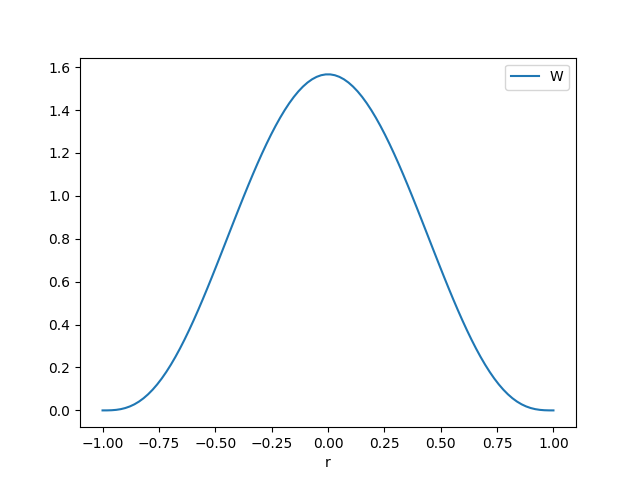
\includegraphics[height=6cm]{compscieng_app40sph_01.png}

\begin{minted}[fontsize=\footnotesize]{python}
df = pd.DataFrame(r)
df.columns = ['r']
df['W'] = (315./(64*np.pi*h**9)) * (h**2 - np.abs(r)**2)**3
df['Gradyan W'] = -945./(32*np.pi*h**9) * r * (h**2 - np.abs(r)**2)**2
df = df.set_index('r')
df.plot()
plt.savefig('compscieng_app40sph_02.png')
\end{minted}

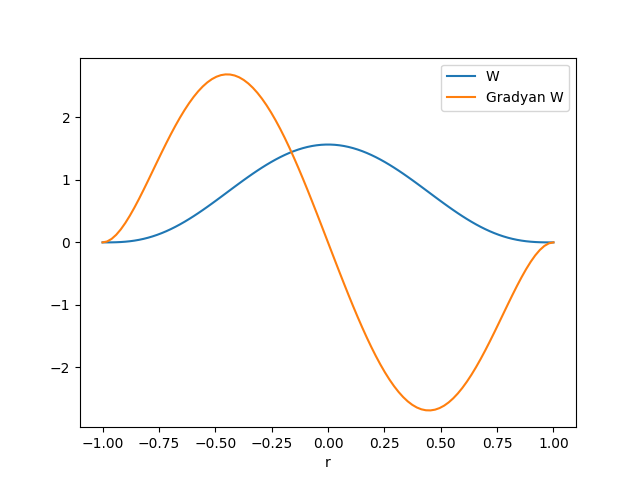
\includegraphics[height=6cm]{compscieng_app40sph_02.png}

\begin{minted}[fontsize=\footnotesize]{python}
df = pd.DataFrame(r)
df.columns = ['r']
df['W'] = (315./(64*np.pi*h**9)) * (h**2 - np.abs(r)**2)**3
df['Gradyan W'] = -945./(32*np.pi*h**9) * r * (h**2 - np.abs(r)**2)**2
df['Laplasyan W'] = -945./(32*np.pi*h**9) * \
                   (h**2-np.abs(r)**2) * \
                   (3*h**2 - 7**np.abs(r)**2)
df = df.set_index('r')
df.plot()
plt.savefig('compscieng_app40sph_03.png')
\end{minted}

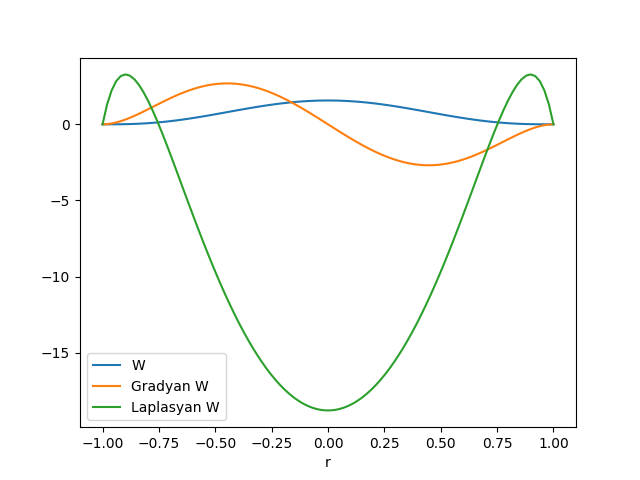
\includegraphics[height=6cm]{compscieng_app40sph_03.png}

Basınç

Basınç kuvveti eğer basınç biliniyorsa hesaplanabilir, basıncın kendisini
hesaplamak için İdeal Gaz Kanunu gerekli [9], bu kanun

$$
p V = n R T
$$

ki $V = 1 / \rho$, yani birim kütleye düşen hacim, $n$ mol üzerinden kaç tane
gaz parçacığı olduğu, $R$ evrensel gaz sabiti, $T$ ise sıcaklık. SPH için sıvıda
eşsıcaklık (isothermal), ve parçacıkların sayısı simulasyon sırasında değişmez
kabul edilir, o zaman üstteki formülün sağ tarafında bir gaz sertlik (stiffness)
sabiti $k$ kullanılabilir [4, sf. 18], 

$$
p V = k
$$

$$
p \frac{1}{\rho} = k
$$

$$
p  = k \rho
$$

Sayısal kodlamalarda stabilite amaçlı olarak ayrıca bir de $\rho_0$ kullanılır,
ki her basınç hesabı için yoğunluğun bu baz $\rho_0$ ile olan farkı bazlı
alınır, nihai formül,

$$
p  = k (\rho - \rho_0)
$$

Simülasyon kodu alttadır. Simüle edilen bir blok sıvıyı havada asılı bir
durumdan bırakmak. Ne olacak? Yerçekim etkisiyle tabii ki sıvı parçacıkları
düşmeye başlayacaklar, ama normal sadece elastik çarpışma içeren simülasyondan
farklı olarak şimdi sıvı parçacıkları arasında ağdalık var, yani birbirlerine
yakın durmaya meyilliler. Ayrıca basınç var, tüm bunların etkisini simüle eden
program acaba sıvısal bir davranış gösterecek mi? Simülasyon animasyon / video
olarak [10]'da bulunabilir, C++ versiyonu \verb!simsph.cpp! dosyasında.

\inputminted[fontsize=\footnotesize]{python}{simsph.py}

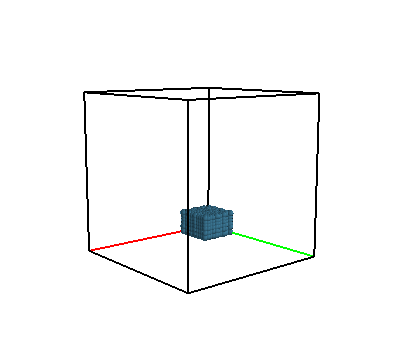
\includegraphics[width=20em]{glutout-002.png}
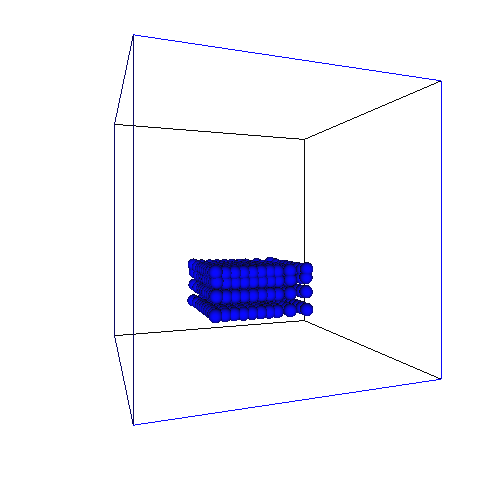
\includegraphics[width=20em]{glutout-004.png}

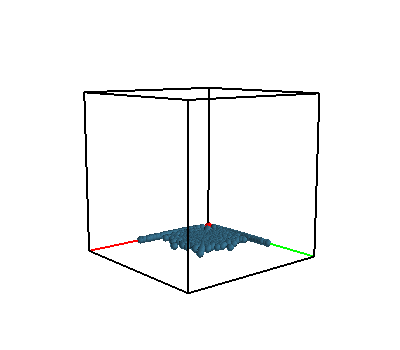
\includegraphics[width=20em]{glutout-006.png}
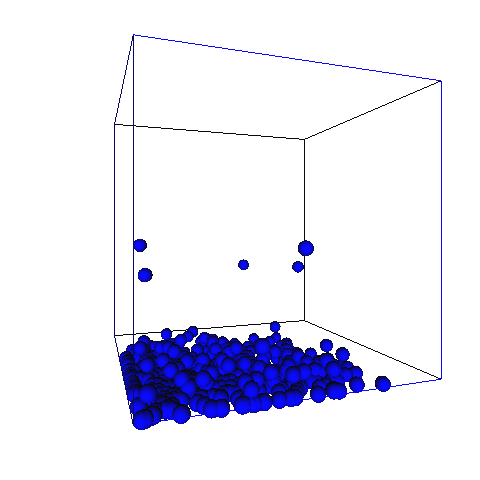
\includegraphics[width=20em]{glutout-008.png}


Kaynaklar

[1] Monaghan, {\em Smoothed particle hydrodynamics, 2005}

[2] Schuermann, {\em Particle-Based Fluid Simulation with SPH},
    \url{https://lucasschuermann.com/writing/particle-based-fluid-simulation}

[3] Bayramlı, {\em Hesapsal Bilim, Ders 4}

[4] Kelager, {\em Lagrangian Fluid Dynamics Using Smoothed Particle Hydrodynamics}

[5] Bayramlı, {\em Fizik, Akış Dinamiği}

[6] Bayramlı, {\em Fizik, Simulasyon}

[7] Monaghan, {\em Introduction to SPH Part I},
    \url{https://www.youtu.be/tAXHCAEgSuE}

[8] Müller, {\em Particle-Based Fluid Simulation for Interactive Applications}

[9] Bayramlı, {\em Fizik, Temel Fizik 3, Basınç, Çarpışma}

[10] Bayramlı, {\em Simulasyon Animasyonu},
    \url{https://github.com/burakbayramli/classnotes/blob/master/compscieng/compscieng_app40sph/balls4.gif?raw=true}

    
\end{document}

